\section{Background}
\label{sec:background}
\shuqing{Maybe we could introduce HID devices somewhere.}
\noindent\outline{USB Standard}\\
We first introduce the development of USB specification and emphasize the key points adopted in our work. We also organized a brief timeline introducing key points of each protocol in Table~\ref{table:usb_timeline}.

\noindent\outline{USB1.x}\\
Proposed in 1996, USB 1.0\cite{usb10} was developed to provide an unified interface and thus reducing the cost of re-configuring the software. It is worth mentioning that as a polled-bus interface, all data transfers are initiated by the host.

\noindent\outline{HID Protocol}\\
Right after one year of the appearance of USB 1.0, a standard named HID (\emph{Human Interface Device})\hongyi{Citation Needed} was born on the basis of USB. HID is designed with the goal of unifying the implementation for devices like mouse, keyboard and so on. Before its appearance, the standard is divided between manufacturers, for example, mouses of Company A may uses X-Y coordinates to represent its location while mouses of Company B uses relative displacement. This means every device needs their own drivers to work. After HID, people just write one driver for an entire class of HIDs. Furthermore, HID standard also requires all devices to be PnP (\emph{Plug-and-Play}), which is indeed convenient but very dangerous too. 

In 1998, the first widely supported USB protocol was born. USB1.1\cite{usb11} provided two data transfer rates which are Low Speed (1.5 Mbit/s) and Full Speed (12 MBit/s). At this point, due to the transfer limit, it only supports limited kinds of devices like keyboard, mice, etc.

\noindent\outline{USB2.0}\\
In 2000, USB 2.0\cite{usb20} specification was released. With High Speed (480 Mbit/s) mode introduced, printer, camera, CD-ROM drive and network cards were supported in this revision. Such high data transfer rate also gave rise to the popularity of ``flash drive'', portable device that allows physically transferring data around \cite{sok}. Though various peripherals were supported in USB 2.0, there was no reliable way to identify the type of a device. This security flaw allowed attacks like BadUSB\cite{rubber}.

\noindent\outline{USB3.x}\\
USB 3.0\cite{usb30} was announced in 2008, with a Super Speed (5 Gbit/s) data transfer rate. Like its predecessor, more classes of peripherals were supported in this revision. In 2013, USB Type-C connector standard was introduced as a part of USB 3.1\cite{usb31}, providing a unified connector type for PowerDelivery (PD), Thunderbolt, DisplayPort and HDMI.  Yet no improvement of security was introduced in 3.x revisions, meaning any device claiming themselves as a monitor can capture the video stream from the host. Exposing such multi-propose connector unprotected is dangerous and allows attacks like our work \tool. In 2017, USB 3.2\cite{usb32} was released, doubling the data transfer rate. (20 Gbit/s)

\noindent\outline{Connector Standard}
\begin{figure}[t]
    \centering
	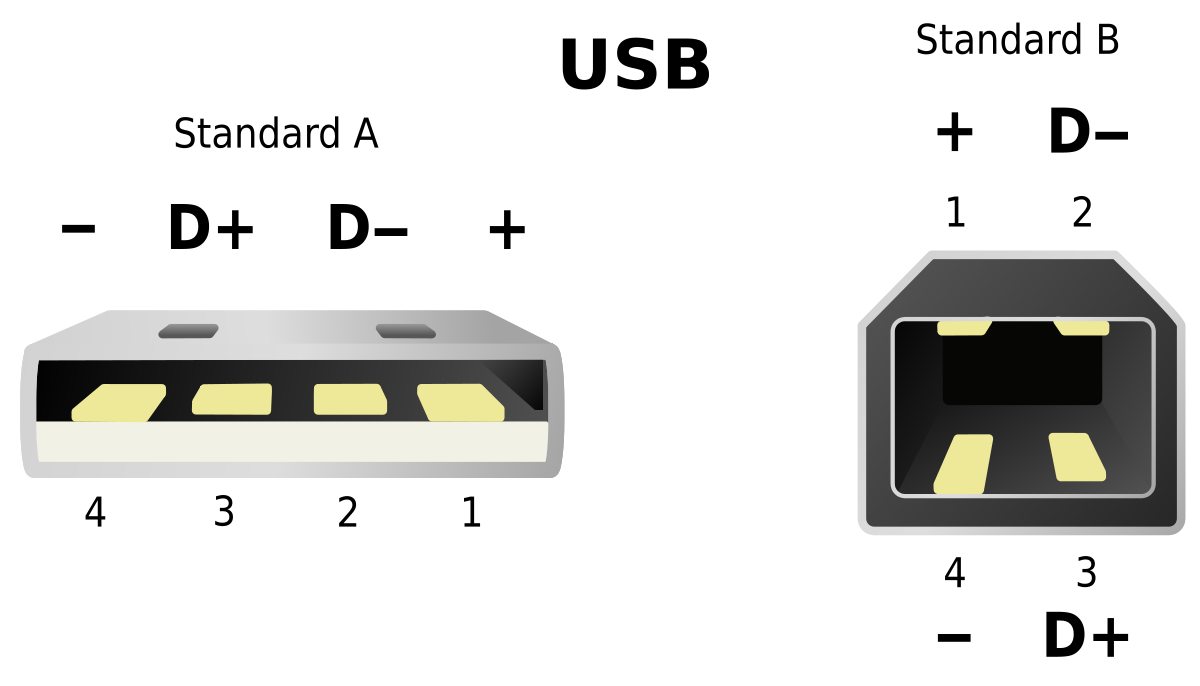
\includegraphics[width=0.7\linewidth]{./Figs/usb_conn.png}
	\caption{USB 1.x \& 2.x Connector}
	\label{fig:usb_conn}
\end{figure}
As illustrated in Figure~\ref{fig:usb_conn}, the original USB 1.x \& 2.x connector only has two pins for data transferring (D+ \& D-), which has significantly limited data transfer rate (5 Gbits/s Max) and support for peripheral like DisplayPort (10.8 Gbit/s Min). Apart from that, support for other peripheral also requires dedicated transferring lane as their standards are not compatible with USB in most cases.
\begin{figure}[t]
	\centering
	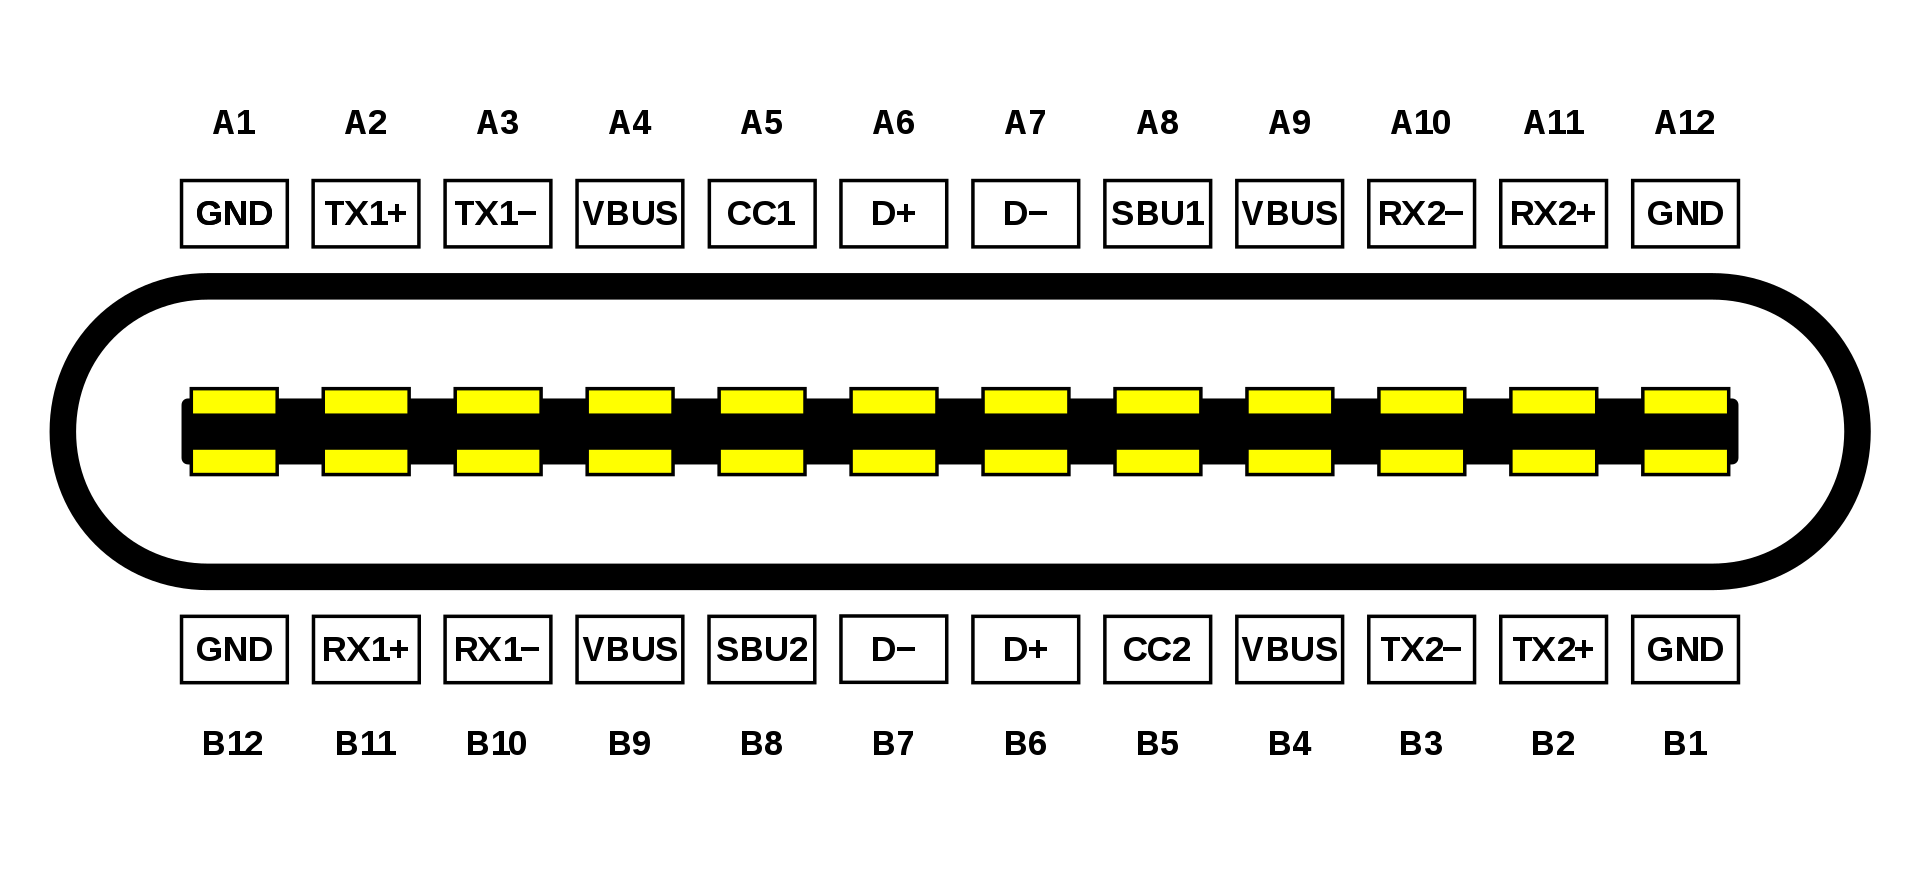
\includegraphics[width=\linewidth]{./Figs/usb_c_conn.png}
	\caption{USB Type C Connector}
	\label{fig:usb_c_conn}
\end{figure}

Thus, in order to provide support towards a wider range of peripherals, a 24-pins standard called USB Type-C is introduced in 2013 by USB-IF. As it is designed to be double-sided, the number of actual usable pins is halved. Nevertheless, this standard has largely enhanced the capability of USB 3.x protocol. As presented in Figure~\ref{fig:usb_c_conn}, Type-C added two high speed data lanes (TRX1 \& TRX2) and kept the original data lane (D+ \& D-). The added lanes are used exclusively to support peripherals like DisplayPort while the kept data lane transfers USB packets.

\noindent\outline{Security Problem}\\
During the development of USB specification, security was rarely considered.  As the USB-IF believes it is the duty of original equipment manufacturers (OEMs) to decide whether security features should be implemented.\hongyi{Citation needed}. But the divergent implementations give a chance for attack like BadUSB\cite{rubber} and our \tool.


\begin{table*}
\begin{tabular}{|c|c|c|c|c|}
	\hline
	Year & Protocol Version & Supported Peripherals & Transfer Speed & Attacks \\
	\hline
	1996 & USB 1.x & Keyboard, Mouse... & 1.5 Mbit/s or 12 Mbit/s & HID Emulating(BadUSB) \\
	\hline
	2000 & USB 2.0 & Flash Drive, High-Definition Link, CD Driver... & 480 Mbit/s & Autorun Attack, Juice Filming Attack \\
	\hline
	2008 & USB 3.0 & / & 5 Gbit/s & / \\
	\hline
	2013 & USB 3.1 & HDMI, DisplayPort, ThunderBolt... & 10 Gbit/s & Armory \\
	\hline
	2017 & USB 3.2 & / & 20 Gbit/s & / \\
	\hline
\end{tabular}
	\linebreak
\caption{USB Protocol Timeline}
\label{table:usb_timeline}
\end{table*}